% Shared standalone design for the editable figure reconstructions.
\documentclass[tikz,border=5pt,10pt]{standalone}
\usepackage[T1]{fontenc}
\usepackage[utf8]{inputenc}
\usepackage{newpxtext,newpxmath}
\usepackage[scaled=.94]{sourcesanspro}
\usepackage{pgfplots}
\pgfplotsset{compat=1.18}
\usetikzlibrary{arrows.meta,calc,positioning,decorations.pathreplacing,
  decorations.markings,patterns,matrix,shapes.geometric,fit,backgrounds,
  intersections,angles,quotes}
\definecolor{ink}{HTML}{203746}
\definecolor{accent}{HTML}{146C78}
\definecolor{muted}{HTML}{667780}
\definecolor{signalred}{HTML}{B94B44}
\color{ink}
\tikzset{>=Latex,line width=.8pt,
  every node/.style={font=\small},
  axis/.style={->,draw=muted,line width=.5pt},
  guide/.style={draw=muted,dashed,line width=.45pt},
  curve/.style={draw=accent,line width=1pt},
  marker/.style={circle,fill=accent,inner sep=1.5pt},
  labelbox/.style={fill=white,inner sep=2pt}}

\begin{document}
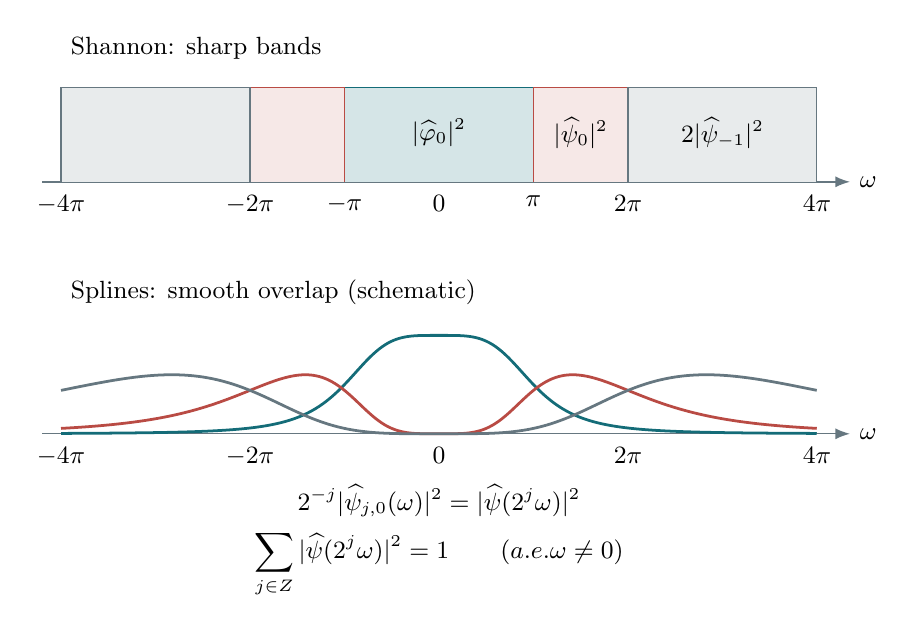
\begin{tikzpicture}[x=1.2cm,y=1cm]
\node[anchor=west] at (-4,3.0) {Shannon: sharp bands};
\draw[axis] (-4.2,1.3)--(4.35,1.3) node[right] {$\omega$};
\fill[accent!18] (-1,1.3) rectangle(1,2.5);\draw[accent] (-1,1.3)--(-1,2.5)--(1,2.5)--(1,1.3);
\foreach \a/\b in {-2/-1,1/2} {\fill[signalred!13] (\a,1.3) rectangle(\b,2.5);\draw[signalred] (\a,1.3)--(\a,2.5)--(\b,2.5)--(\b,1.3);}
\foreach \a/\b in {-4/-2,2/4} {\fill[muted!15] (\a,1.3) rectangle(\b,2.5);\draw[muted] (\a,1.3)--(\a,2.5)--(\b,2.5)--(\b,1.3);}
\node at (0,1.92) {$|\widehat\varphi_0|^2$};\node at (1.5,1.92) {$|\widehat\psi_0|^2$};\node at (3,1.92) {$2|\widehat\psi_{-1}|^2$};
\foreach \x/\lab in {-4/{-4\pi},-2/{-2\pi},-1/{-\pi},0/0,1/\pi,2/{2\pi},4/{4\pi}} {\node[below] at (\x,1.25) {$\lab$};}
\node[anchor=west] at (-4,-.1) {Splines: smooth overlap (schematic)};
\draw[axis] (-4.2,-1.9)--(4.35,-1.9) node[right] {$\omega$};
\draw[curve,domain=-4:4,samples=241] plot (\x,{-1.9+1.25/(1+(\x)^4)});
\draw[signalred,line width=1pt,domain=-4:4,samples=241] plot (\x,{-1.9+1.25*(1/(1+(\x/2)^4)-1/(1+(\x)^4))});
\draw[muted,line width=1pt,domain=-4:4,samples=241] plot (\x,{-1.9+1.25*(1/(1+(\x/4)^4)-1/(1+(\x/2)^4))});
\foreach \x/\lab in {-4/{-4\pi},-2/{-2\pi},0/0,2/{2\pi},4/{4\pi}} {\node[below] at (\x,-1.95) {$\lab$};}
\node at (0,-2.75) {$2^{-j}|\widehat\psi_{j,0}(\omega)|^2=|\widehat\psi(2^j\omega)|^2$};
\node at (0,-3.55) {$\displaystyle\sum_{j\in\mathbb Z}|\widehat\psi(2^j\omega)|^2=1\qquad(\text{a.e. }\omega\ne0)$};
\end{tikzpicture}
\end{document}
